%! Author = sbbfti
%! Date = 10/06/2020


\section{Results}\label{sec:results}

The sensible heat loss from the skin to the environment is proportional to the difference between the \ac{t-sk} and \ac{t-op}, as shown in Equation~\ref{eq:c-r}.
Consequently, for values of \ac{t-op} higher than \ac{t-sk} the body gains sensible heat from its environment and the term \ac{c-r} becomes negative.
Figure~\ref{fig:comparison_models}A shows how the sensible heat loss estimated with the \mycite{GaggeSET} and the \mycite{Jay2015} models vary as a function of \ac{t-op}, \ac{rh}, and \ac{v}.
The former model iteratively determines \ac{t-sk}, while the latter assumes it to be constant and equal to 35~$^{\circ}$C\@.
When heat gains exceed heat losses, the \mycite{GaggeSET} model estimates that some heat energy gets stored in the body and consequently \ac{t-sk} increases, as shown in Figure~\ref{fig:results_model_2}A and ~\ref{fig:results_model_2}C, respectively.
This reduces the rate at which sensible heat gain increases as \ac{t-op} increases.

The values of \ac{w} and the respective values of \ac{w-max} for two air speeds are shown in Figure~\ref{fig:comparison_models}B\@.
For young adults, \mycite{Jay2015} assumed \ac{w-max} to be equal to 0.65 for the `fan on' condition and 0.85 for the `fan off' condition.
In the \mycite{GaggeSET}, the value of \ac{w-max} only changes as a function of \ac{v}.
It can be observed that the critical operative temperature at which \ac{w} equals \ac{w-max} is a inversely proportional to the value of \ac{rh}.

\begin{figure}[thb!]
    \centering
    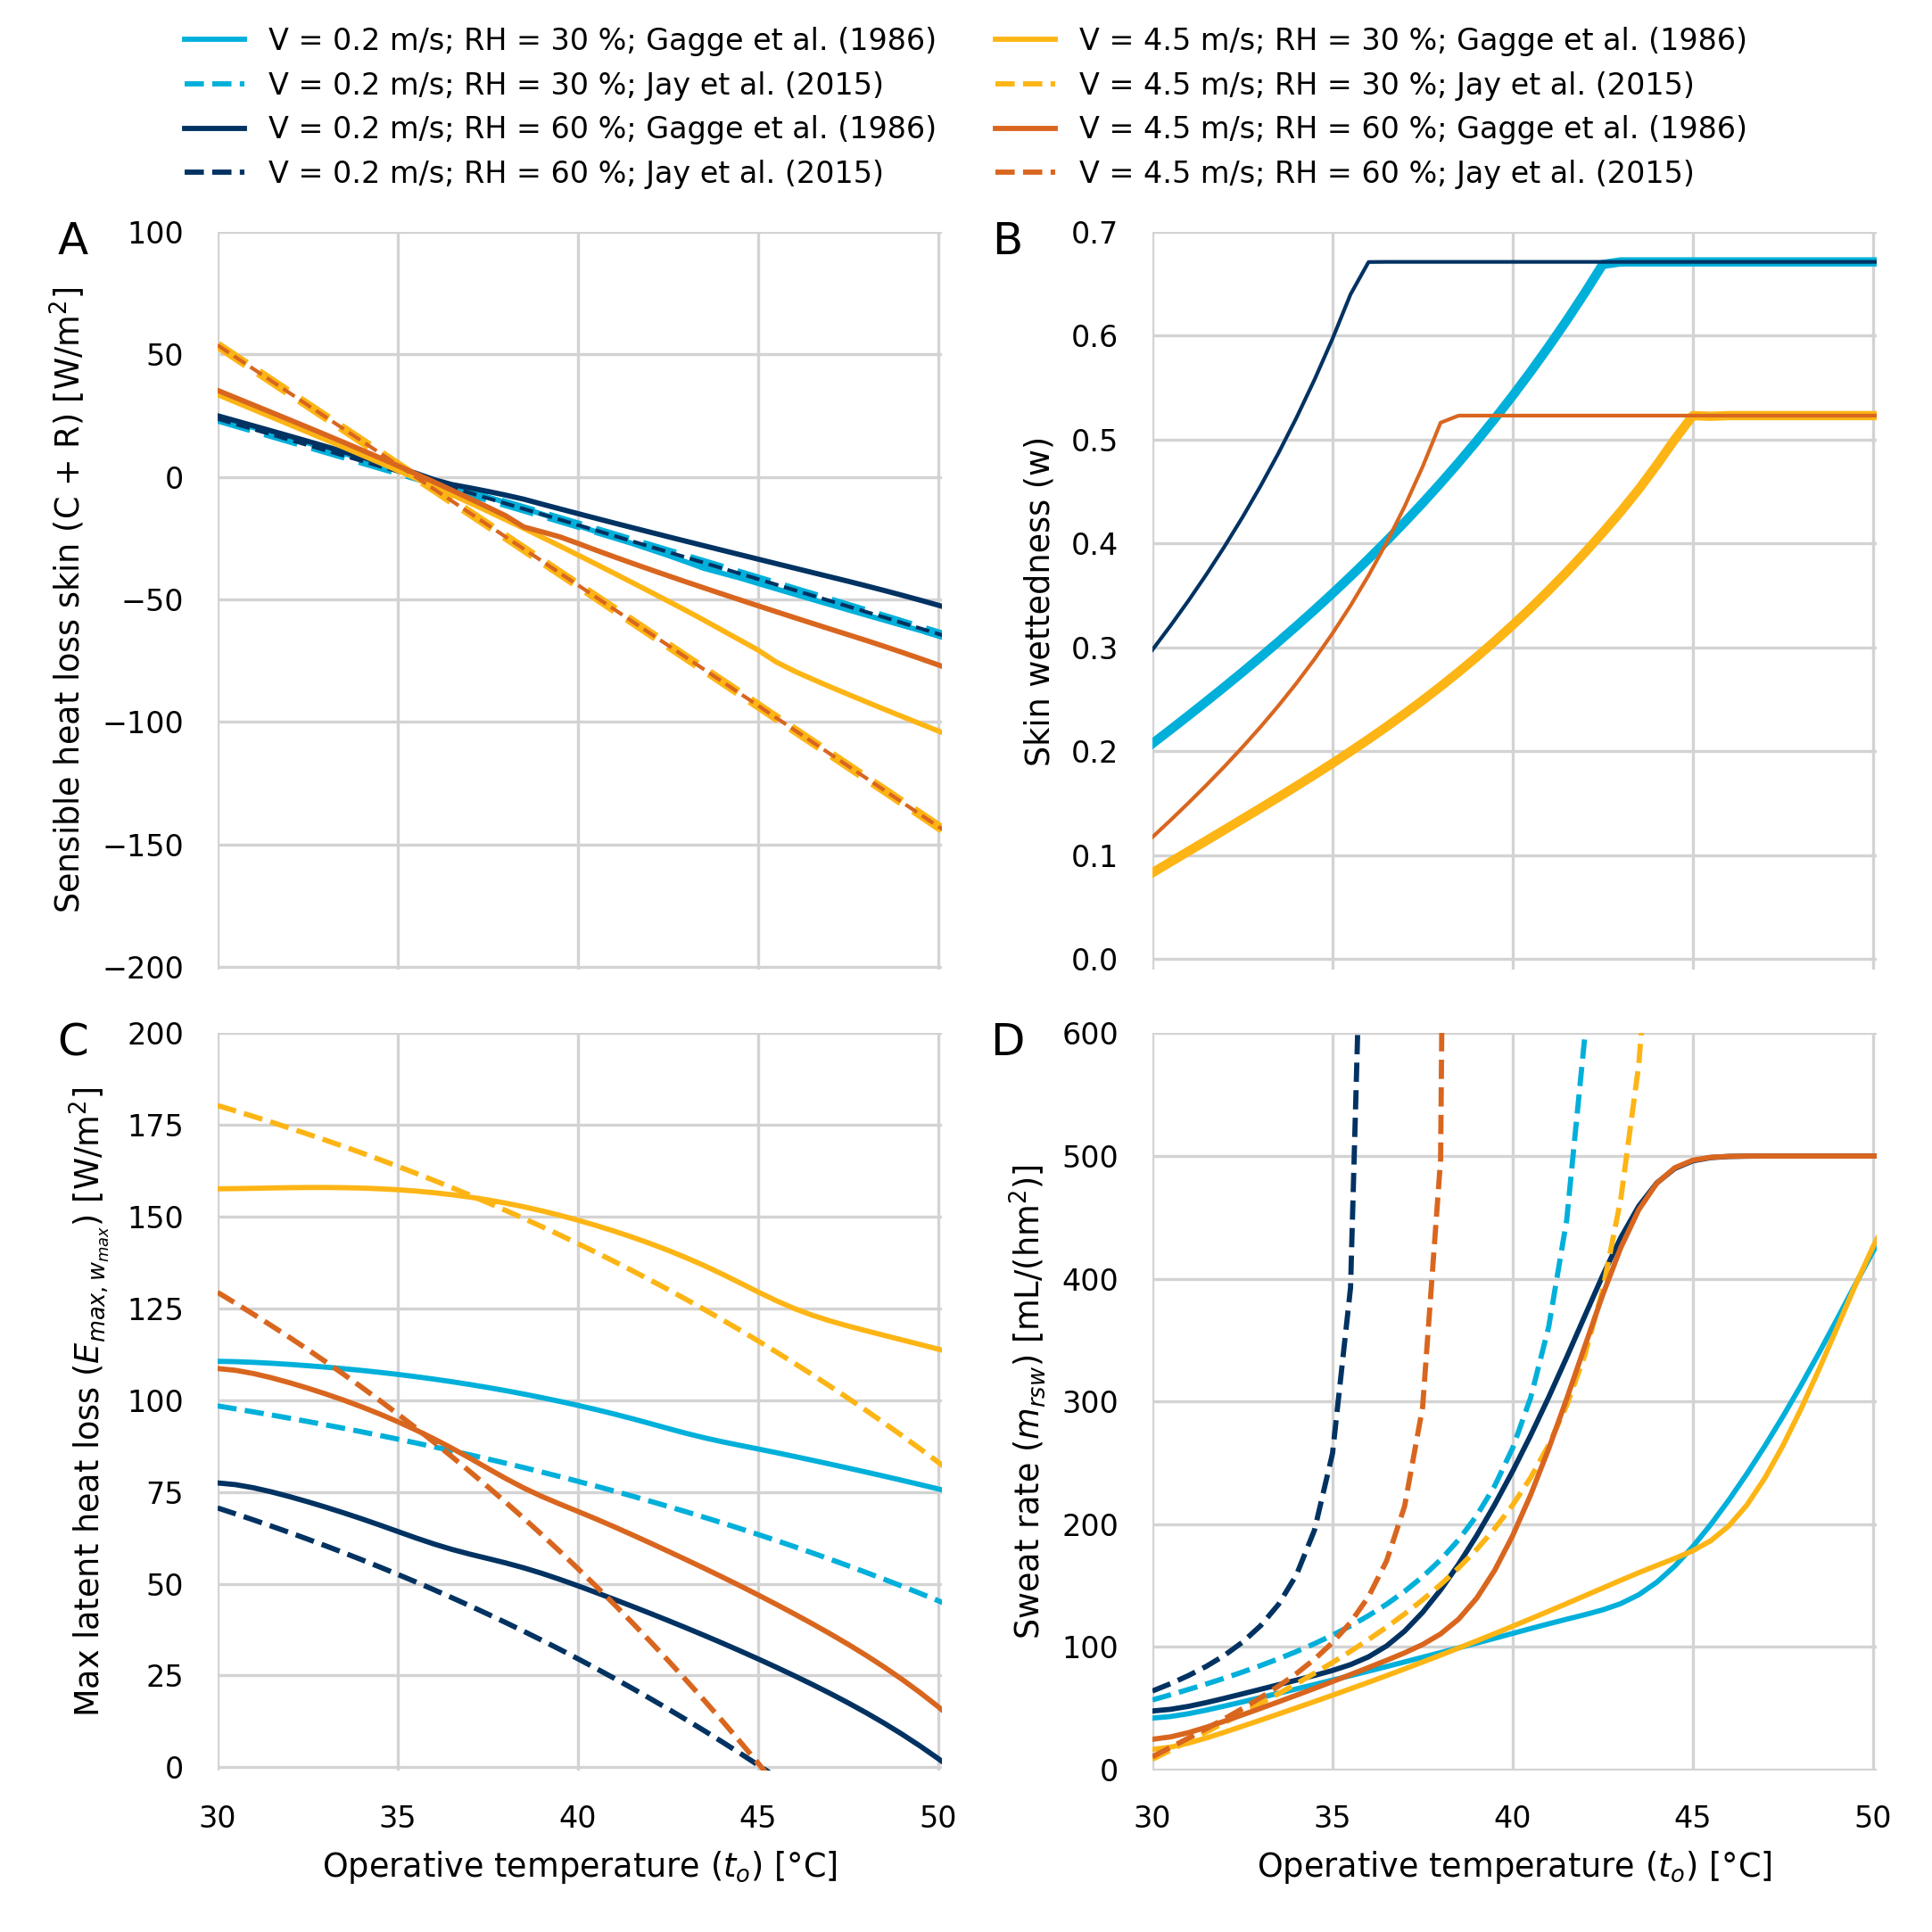
\includegraphics[width=\textwidth]{figures/comparison_models_v2.png}
    \caption{Results obtained with the the energy models proposed by \mycite{Jay2015} and \mycite{GaggeSET}.
    Each Figure shows how a variable changes as a function of \ac{t-op} for a set combination of \ac{rh} and \ac{v}.
    Figure A - Sensible heat loss from the skin.
    Figure B - Skin wettendess.
    Figure C - Maximum latent heat loss estimated using \ac{w} = \ac{w-max}.
    Figure D - Sweat rate.}
    \label{fig:comparison_models}
\end{figure}

% todo Stefano - this figure requires several improvements. - It is too complex and you should select only the most important cases,. If it is not fundamental, just mention that people can explore in the tool. - the Jay lines should be dotted not line and dot. - if the line overlaps, you need to manually draw next to is so it can be seen, otherwise only one line is shown and some researchers could get confused. -add Jay skin wetteness to Figure b, even if fix. - you must chose the color from a different pallet.

% todo remove w_crit Jay

For \ac{t-op} higher than \ac{t-sk}, the negative effect that an increase in \ac{v} has on sensible heat gain is compensated by a greater increase in the \acf{e-sk} that the body can dissipate towards the surrounding environment.
For example, when \ac{t-op}~=~45~$^{\circ}$C and \ac{rh}~=~30~\%, an increase in \ac{v} from 0.2 to 4.5~m/s increases the sensible heat gains (\acs{c-r}) by 29 W/m\textsuperscript{2} while increasing \ac{e-sk} by 45~W/m\textsuperscript{2}, hence, increasing \ac{v} has a net positive effect.

Figure~\ref{fig:comparison_models}C shows the values of \ac{e-max} estimated by replacing \ac{w} in Equation~\ref{eq:latent-skin} with \ac{w-max}.
The value of \ac{e-max} decreases as \ac{t-op} increases since \ac{p-a} grows more rapidly than \ac{p-sk}.
For a set combination of \ac{v} and \ac{t-op} the value of \ac{e-max} decreases as the value of \ac{rh} increases.
This is because humid air has a higher \ac{p-a} than dry air.
The reduction in \ac{e-max} estimated by our model is lower than the one estimated by \mycite{Jay2015} since an increase in \ac{t-sk} elevates the vapor pressure gradient between the skin and the surrounding environment.

The \acf{m-sweat} is shown in Figure~\ref{fig:comparison_models}D\@.
The difference between the results obtained with the two heat balance models can be attributed to the fact that \citeauthor{Jay2015} calculate the value of \ac{m-sweat} as a function of the required latent energy that the body should in theory dissipate to achieve thermal neutrality.
On the other hand, \citeauthor{GaggeSET} calculate the value of \ac{m-sweat} as a function of regulatory signals and they assume that \ac{m-sweat} cannot exceed 500~mL/h.
% note In the most recent paper from Jay, they assume that the max sweat rate is 440 mL/h (in their model). However, we can sweat more than 500 mL/h, for example in a field study participants exposed to 47C and 10%  sweated 691 mL/h (when fan were on) but when fan off they sweated 328g/h. Under 40C and 50% they sweated 346 and 216 g/h, with fan and no fan, respectively.  Hence, only with very low humidity, high temp and fan  on people sweated more than 500. I do not know what it the max value we can sweat, I guess it would vary from person to person. Moreover, Gagge's model estimates that the a value of 500mL/h is only reached in extreme conditions (red area Figure 7) when fans should no longer be used. I am planning to add a table at the end of the 

\begin{figure}[thb!]
    \centering
    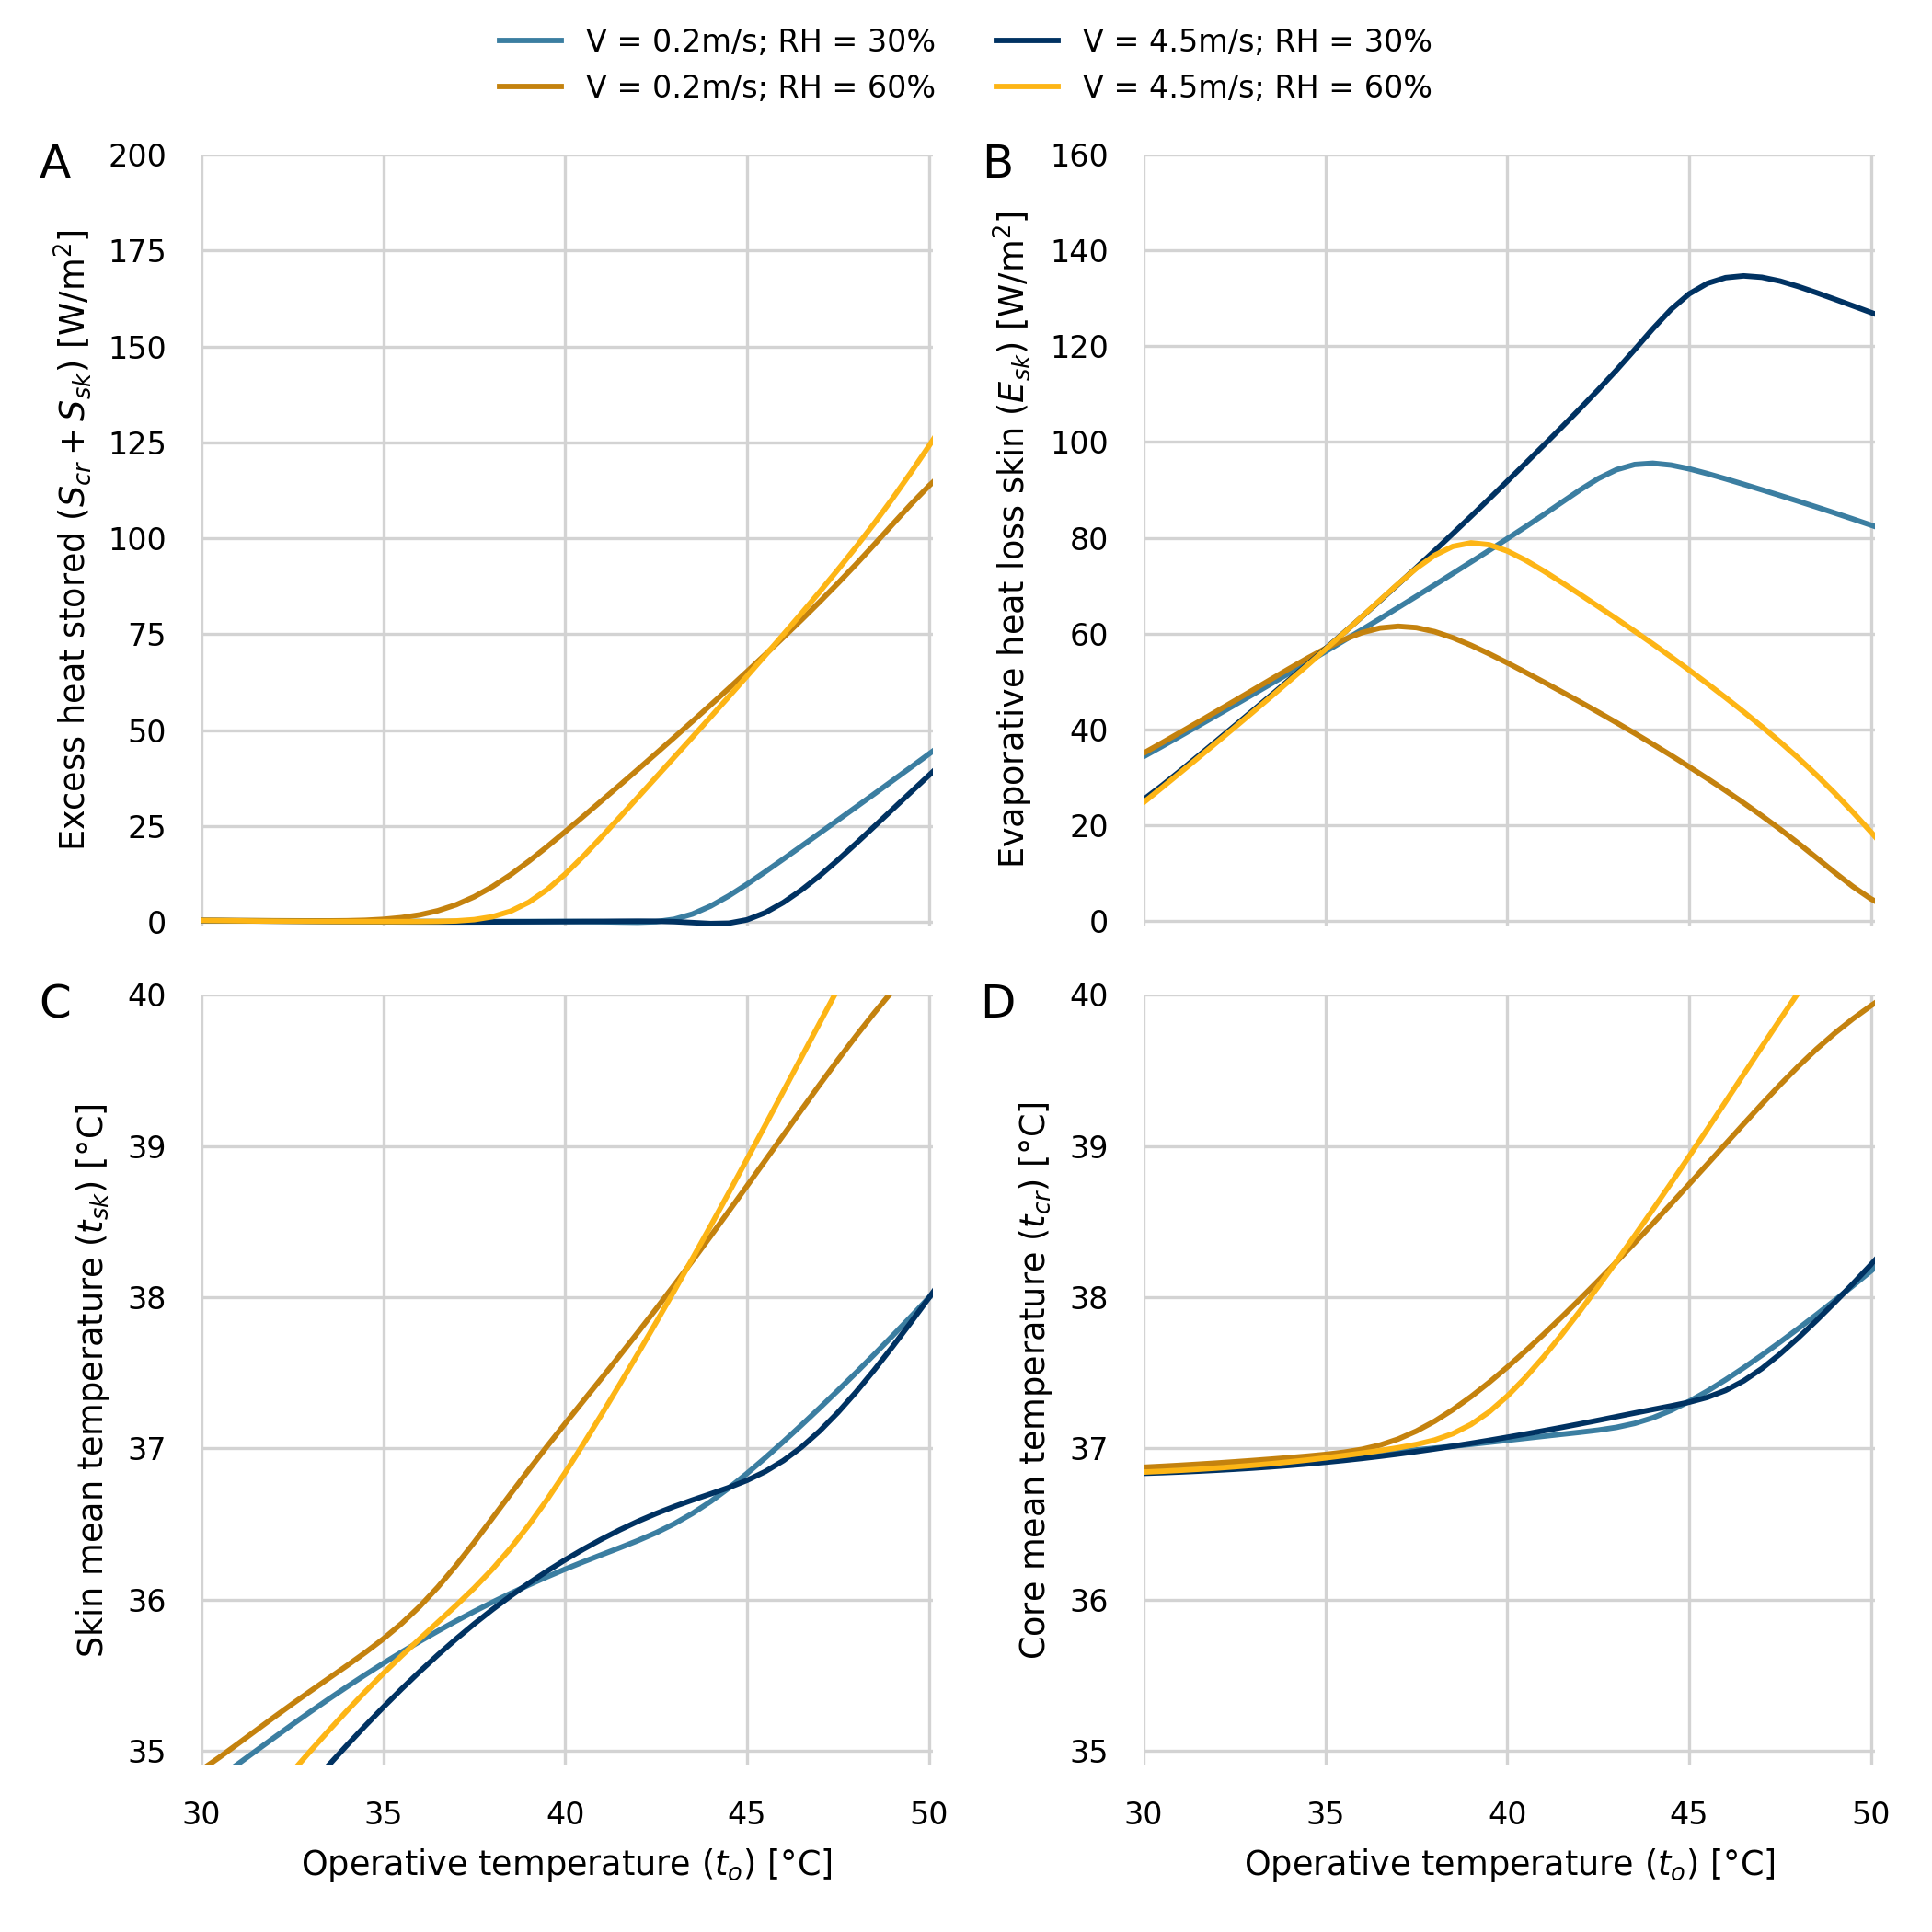
\includegraphics[width=\textwidth]{figures/results_model_2}
    \caption{Results obtained with \mycite{GaggeSET} energy model.
    Each Figure shows how a variable changes as a function of \ac{t-op} for a set combination of \ac{rh} and \ac{v}.
    Figure A - Excess heat stored in the human body, skin and core compartments, \ac{s-sk} + \ac{s-cr}.
    Figure B - Evaporative hear loss via the skin, \ac{e-sk}.
    Figure C - Skin mean temperature, \ac{t-sk}.
    Figure D - Core mean temperature, \ac{t-cr}.}
    \label{fig:results_model_2}
\end{figure}

The excess heat stored in the human body (\acs{s-cr} + \acs{s-sk}), \ac{t-sk}, and \ac{t-cr} are shown in Figure~\ref{fig:results_model_2}A, ~\ref{fig:results_model_2}C, and ~\ref{fig:results_model_2}D, respectively.
When the body cannot longer dissipate exogenous and endogenous heat gains, the excess heat gets stored in the human body causes \ac{t-sk} and \ac{t-cr} to raise.

% note: The increase in the core temperature it is a concern, but as you can see from Figure 3 if the fans are on, the increase in core body temperature is smoother than when fans are off. This is true till a certain point when this trend is inverted and the core temperature with the fans on is higher than with the fan off. As you can see from Figure 3 the point in which the two lines intersect is the same point above which in Figure 7 we are no longer recommending to use electrical fans. Hence, fans are still beneficial to use, even though people may be suffering a bit, they are better than nothing. Moreover, from figure 3 it can be observed that the critical temperature above which core body temperature starts increasing is higher when fans are turned on, and this temperature is higher than 35C. Till that temperature the use of fans is actually good since it onset the increase in the core temperature.

The combination of \ac{t-op}, \ac{rh}, and \ac{v} at which heat stress would start to occur is presented in Figure~\ref{fig:comparison_air_speed}.
Each line demarcates the region in which thermal stress is estimated to occur.
Above this line not all individuals would be able to compensate for endogenous and exogenous heat gains.
The Figure shows the results obtained with both the \mycite{GaggeSET} and the \mycite{Jay2015} models.
For a specific value of \ac{v}, the maximum \ac{t-op} at which cardiovascular strain is estimated to occur decreases as the value of \ac{rh} increases.
In addition, it can be observed that for a specific value of \ac{rh}, as the value of \ac{v} increases the overall increase in the maximum critical temperature rapidly decreases.
For example, in an environment with \ac{rh}~=~60~\%, increasing \ac{v} from 0.2~m/s to 0.8~m/s then to 4.5~m/s lead to an increase of the critical temperature of approximately 2.3~$^{\circ}$C and 0.8~$^{\circ}$C, respectively.

In Figure~\ref{fig:comparison_air_speed} we are also presenting the results obtained by \mycite{Morris2019} and \mycite{Rate2015}.
The former determied that eletric fans (\ac{v}~=~2.0~m/s) are beneficial when \ac{t-db}~=~42~$^{\circ}$C and \ac{rh}~=~50~\%, but should not be used when \ac{t-db}~=~36~$^{\circ}$C and \ac{rh}~=~80~\%.
While \mycite{Rate2015} concluded that electric fans (\ac{v}~=~4.0~m/s) help in preventing heat-related elevation in heart rate and \ac{t-cr} in both of the following conditions \ac{t-db}~=~42~$^{\circ}$C and \ac{rh}~=~50~\%, and \ac{t-db}~=~36~$^{\circ}$C and \ac{rh}~=~80~\%.
The black dashed lines are isoenthalpic lines passing through the conditions studied by \mycite{Morris2019}.
\mycite{Morris2019} concluded that fans are beneficial in hot and humid conditions, but should not be used in hot and dry conditions.
The results of the heat balance model we used in this paper led to similar conclusions to those found experimentally in the two aforementioned studies.
The slope of the heat stress curve flattens for values of \ac{rh} lower than 20 \%.
This can be explained by the fact, not shown in the figures, that for low values of \ac{rh} skin blood flow reaches its upper threshold causing thermal strain.
Our model, appears to slightly underestimate this effect when our results are compare with those obtained by \mycite{Morris2019}.
Our results show that electrical fans should not be used for \ac{rh} lower than 10~\% and \ac{t-db} higher than 49~$^{\circ}$C\@, which is where the gray solid line intercepts the yellow line.
It should, however, be noted that, as previously mentioned in the Introduction Section, in the aforementioned hot and dry condition air enthalpy is lower than in the hot and humid condition (i.e. \ac{t-db}~=~40~$^{\circ}$C and \ac{rh}~=~51~\%).
Evaporative cooling technologies can, therefore, be used to reduce skin blood flow and avoid heat strain.
Evaporative cooling can be achieved by spraying water in the air or even by placing wet towels near the electric fan.
On the other hand, our model slightly underestimate the results obtained by \mycite{Rate2015}, since empirical evidence has shown that the use of electrical fans would still be beneficial even in more extreme heat events.
This difference may be partially explained by some of the conservative assumption we selected, such as, assuming a clothing level of \ac{clo} = 0.5 clo.
\mycite{Rate2015} in their manuscript did not report the clothing level of the participants.

% todo Remove the points from the experimental studies and show them in Figure 7 were it is easier to compare our results with the experimental data.

% todo You tend to overload the figure with too much infomartion. I suggest to: - remove the isoenthalphy lines - remove the 0.8 m/s gagge line. I know that you need to make the point about the uselessness of high air speed, but you can do verbally without the line. - in other figure you had top in the x-axis, why did you change that?, -the figure size ratio (x/y is >1) tend to compress Y a lot, why not plot it as a square (x/y=1)? The plot ratio should represent the importance of the variable. If Top is more important than RH, then x/y<1.

% todo remove isoenthalpic lines from the caption as well

\begin{figure}[thb!]
    \centering
    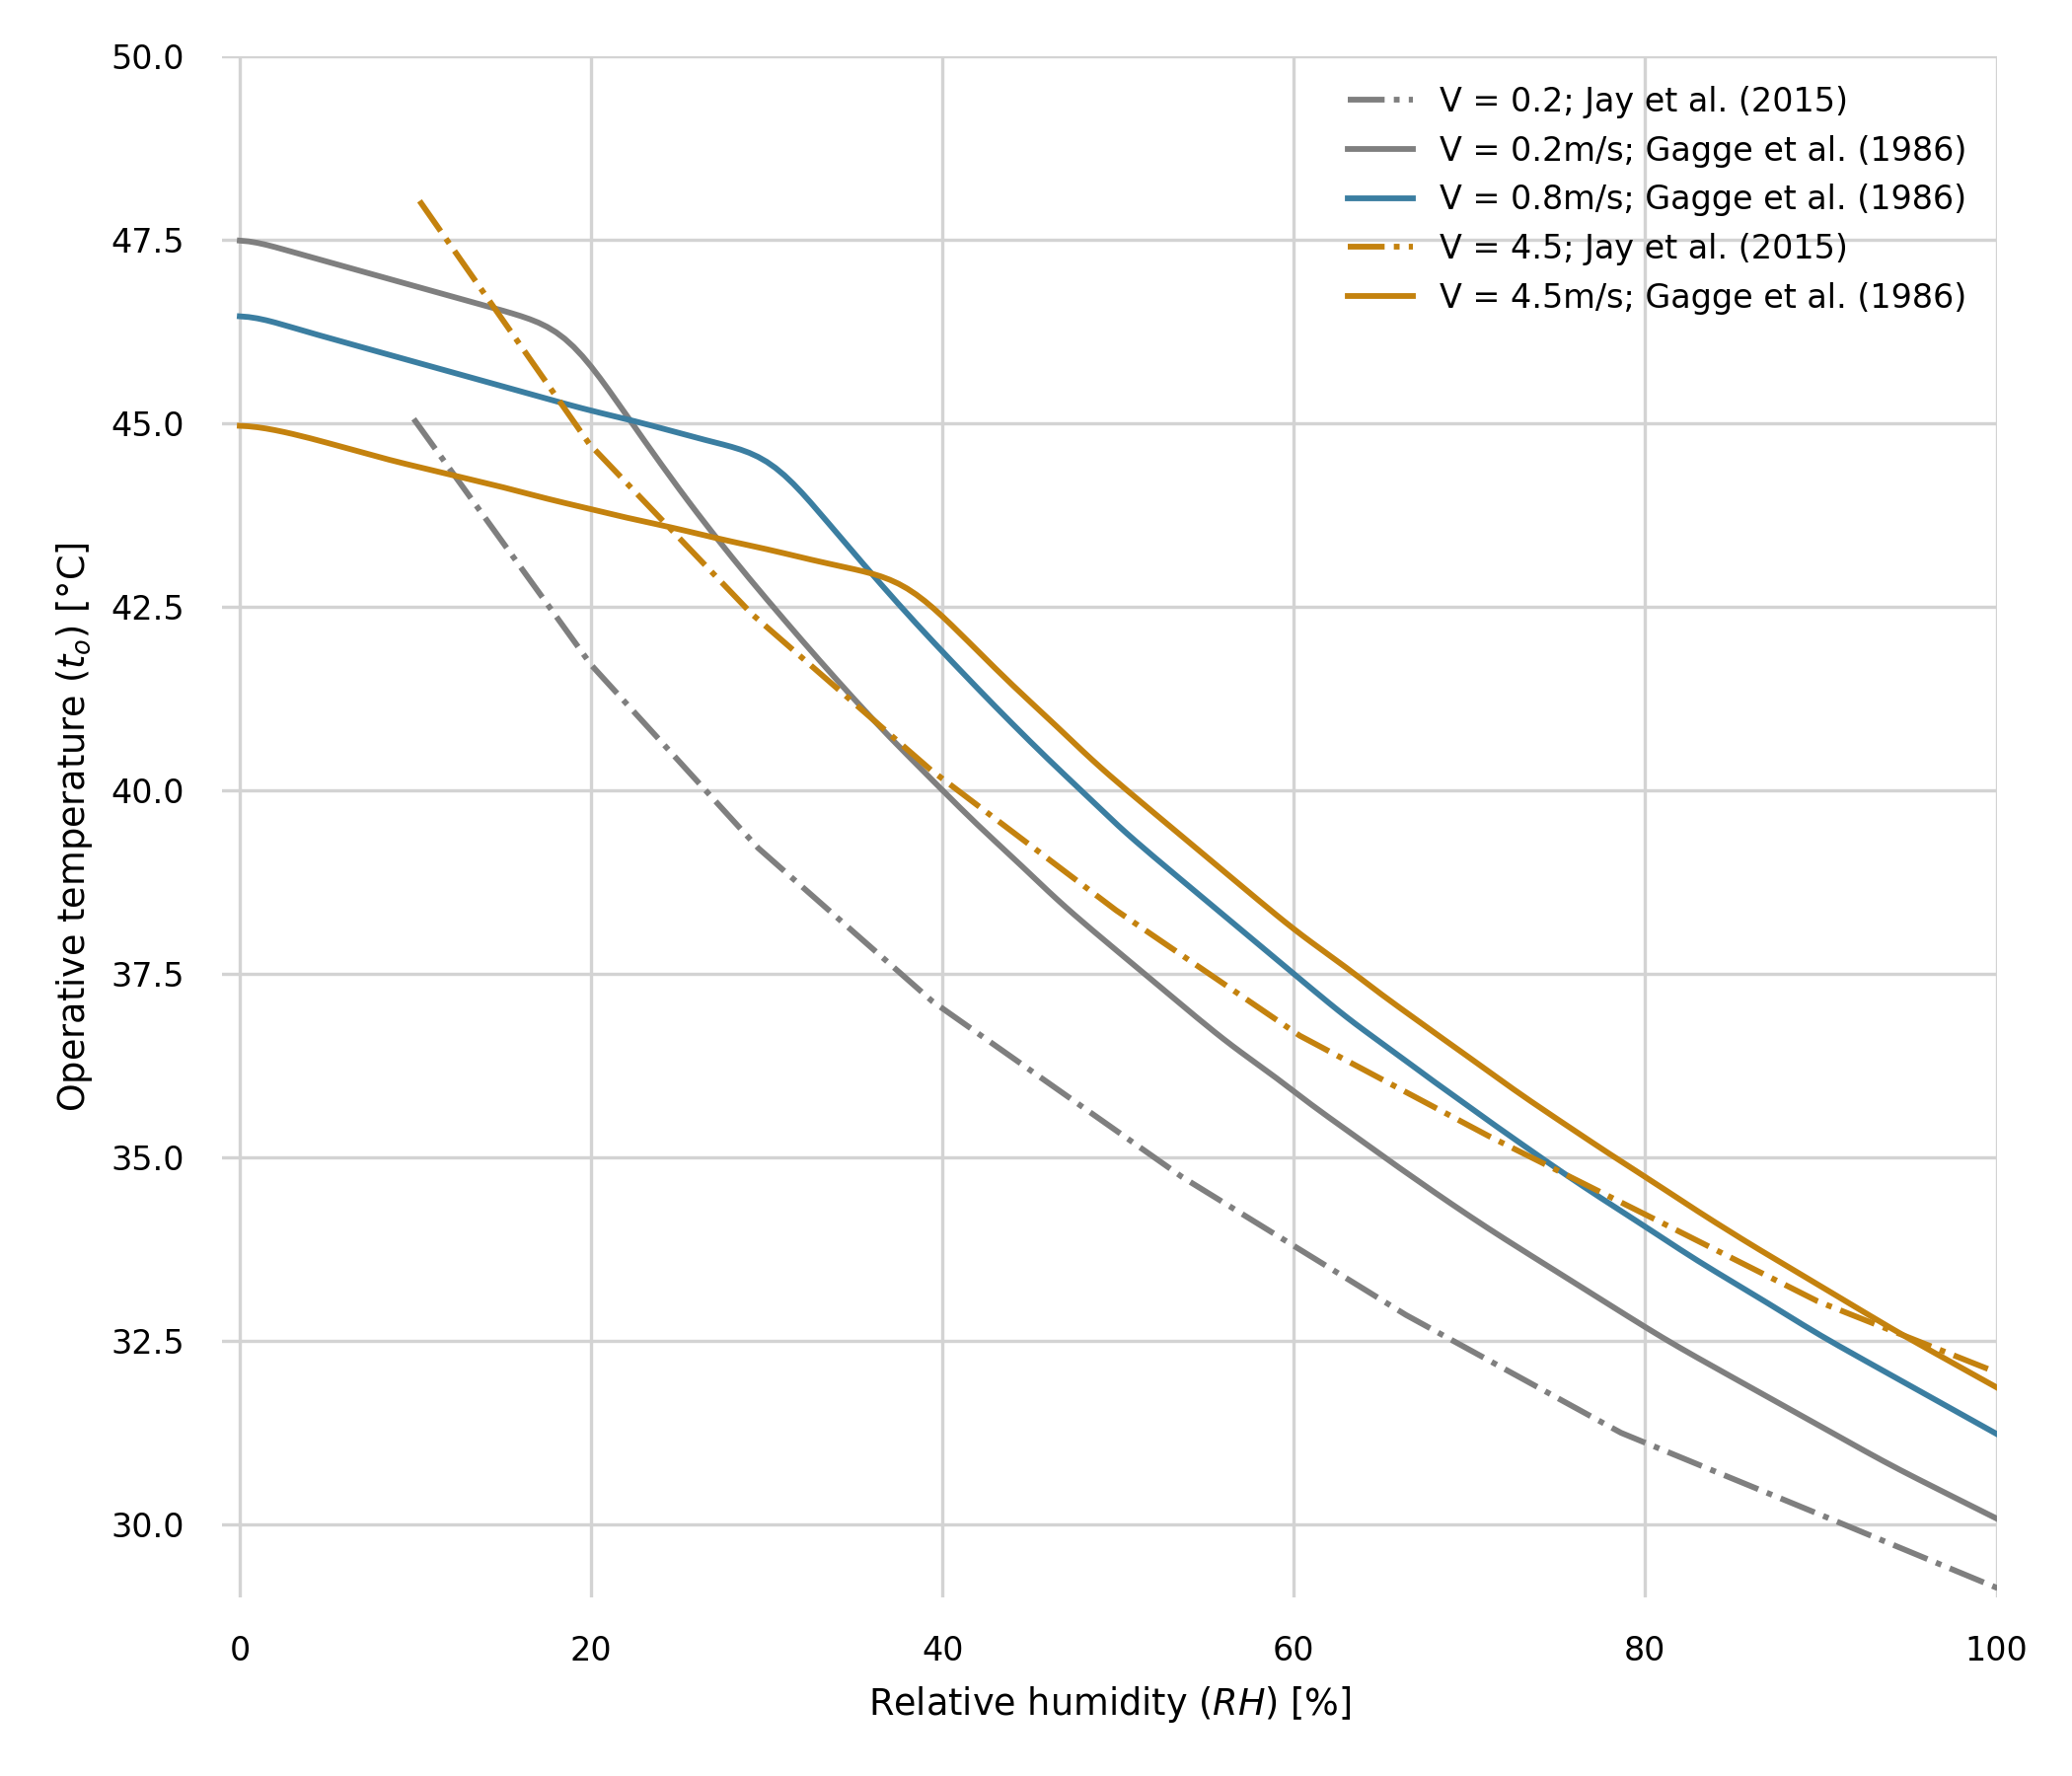
\includegraphics[width=\textwidth]{figures/comparison_air_speed.png}
    \caption{Predicted limits above which thermal strain is estimated to occur.
    The figure shows the results calculated using the \mycite{GaggeSET} model and the \mycite{Jay2015} models.
    In addition, we are presenting the experimental results obtained by \mycite{Morris2019} and \mycite{Rate2015}.
    The solid and dash dotted lines demarcate the point above which heat strain is expected to occur.
    The dashed lines are isoenthalpic lines, which show the enthalpy of the two conditions studied by \mycite{Morris2019}}
    \label{fig:comparison_air_speed}
\end{figure}

To further validate the results of our model, we decided to plot how the predicted value of \ac{t-cr} would vary as a function of \ac{rh}, under a set of specific conditions as tested experimentally by \mycite{Rate2015} (e.g., \ac{t-db}~=~42~$^{\circ}$C, \ac{v}~=~4.0~m/s, \ac{clo}~=~0.35~clo, and \ac{met}~=~1.0~met).
The results are shown in Figure~\ref{fig:comparison_ravanelli}.
It should be noted that \mycite{Rate2015} only reported the core body temperature of one participant.
Consequently, despite the our predicted values are in agreement with their experimental data (mean absolute error~=~0.04~$^{\circ}$C), more quantitative data are needed to validate our results.

\begin{figure}[thb!]
    \centering
    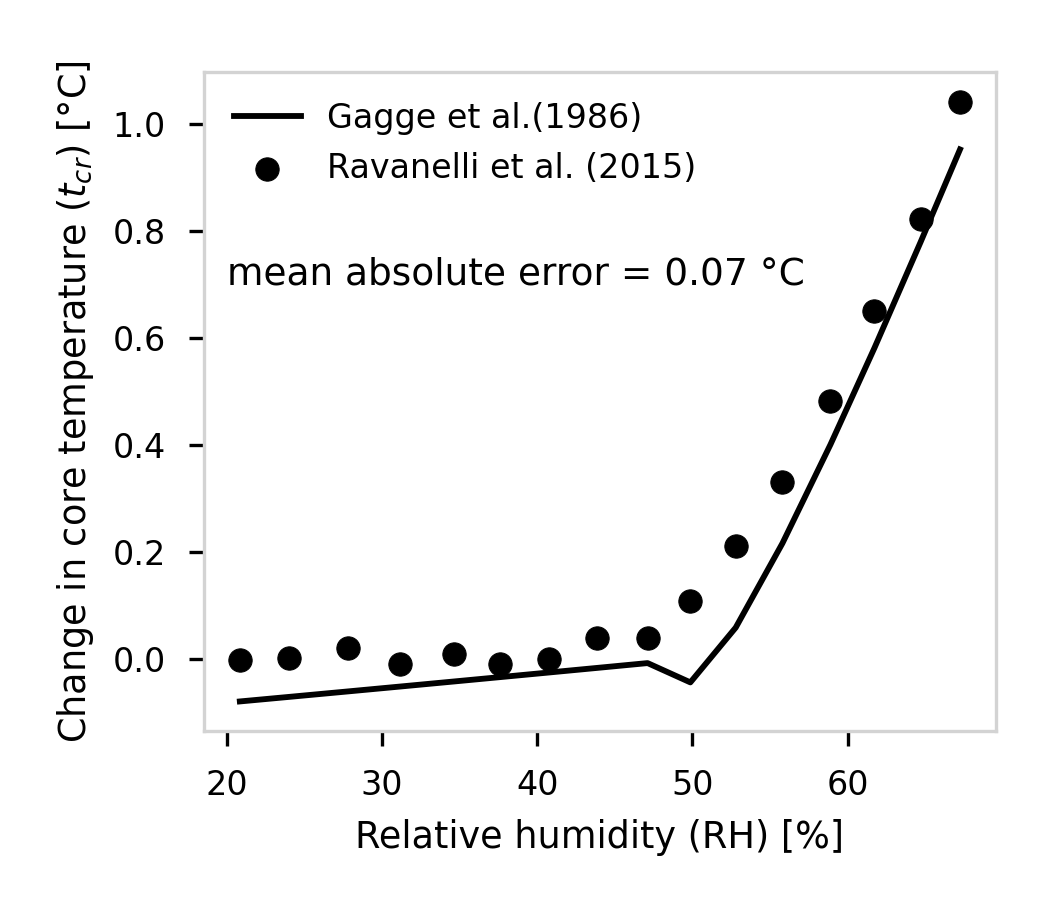
\includegraphics[width=0.5\textwidth]{figures/comparison_ravanelli}
    \caption{Change in \acf{t-cr} as a fuction of \acf{rh}.
    Where \ac{t-db}~=~42~$^{\circ}$C and \ac{v}~=~4.0~m/s.
    The figure shows the results calculated using the \mycite{GaggeSET} model and those obtained experimentally by \mycite{Rate2015}.}
    \label{fig:comparison_ravanelli}
\end{figure}

To better understand how personal factors would impact the body ability to dissipate heat, we calculated when heat stress would occur for different combinations of \ac{met} and \ac{clo}.
Results for people wearing light summer clothing (walking shorts, short-sleeve shirt and sandals, \acs{clo} = 0.36 clo), and office summer clothing (trousers, short-sleeve shirt, and closed shoes \acs{clo} = 0.5 clo) who are either seated reading or writing (\ac{met} = 1.0 met) or standing relaxed (\ac{met} = 1.2 met) are shown in Figure~\ref{fig:met_clo}.
As expected, decreasing both \ac{met} and \ac{clo} has a net positive effect since it reduces both heat gains and thermal resistance.

\begin{figure}[thb!]
    \centering
    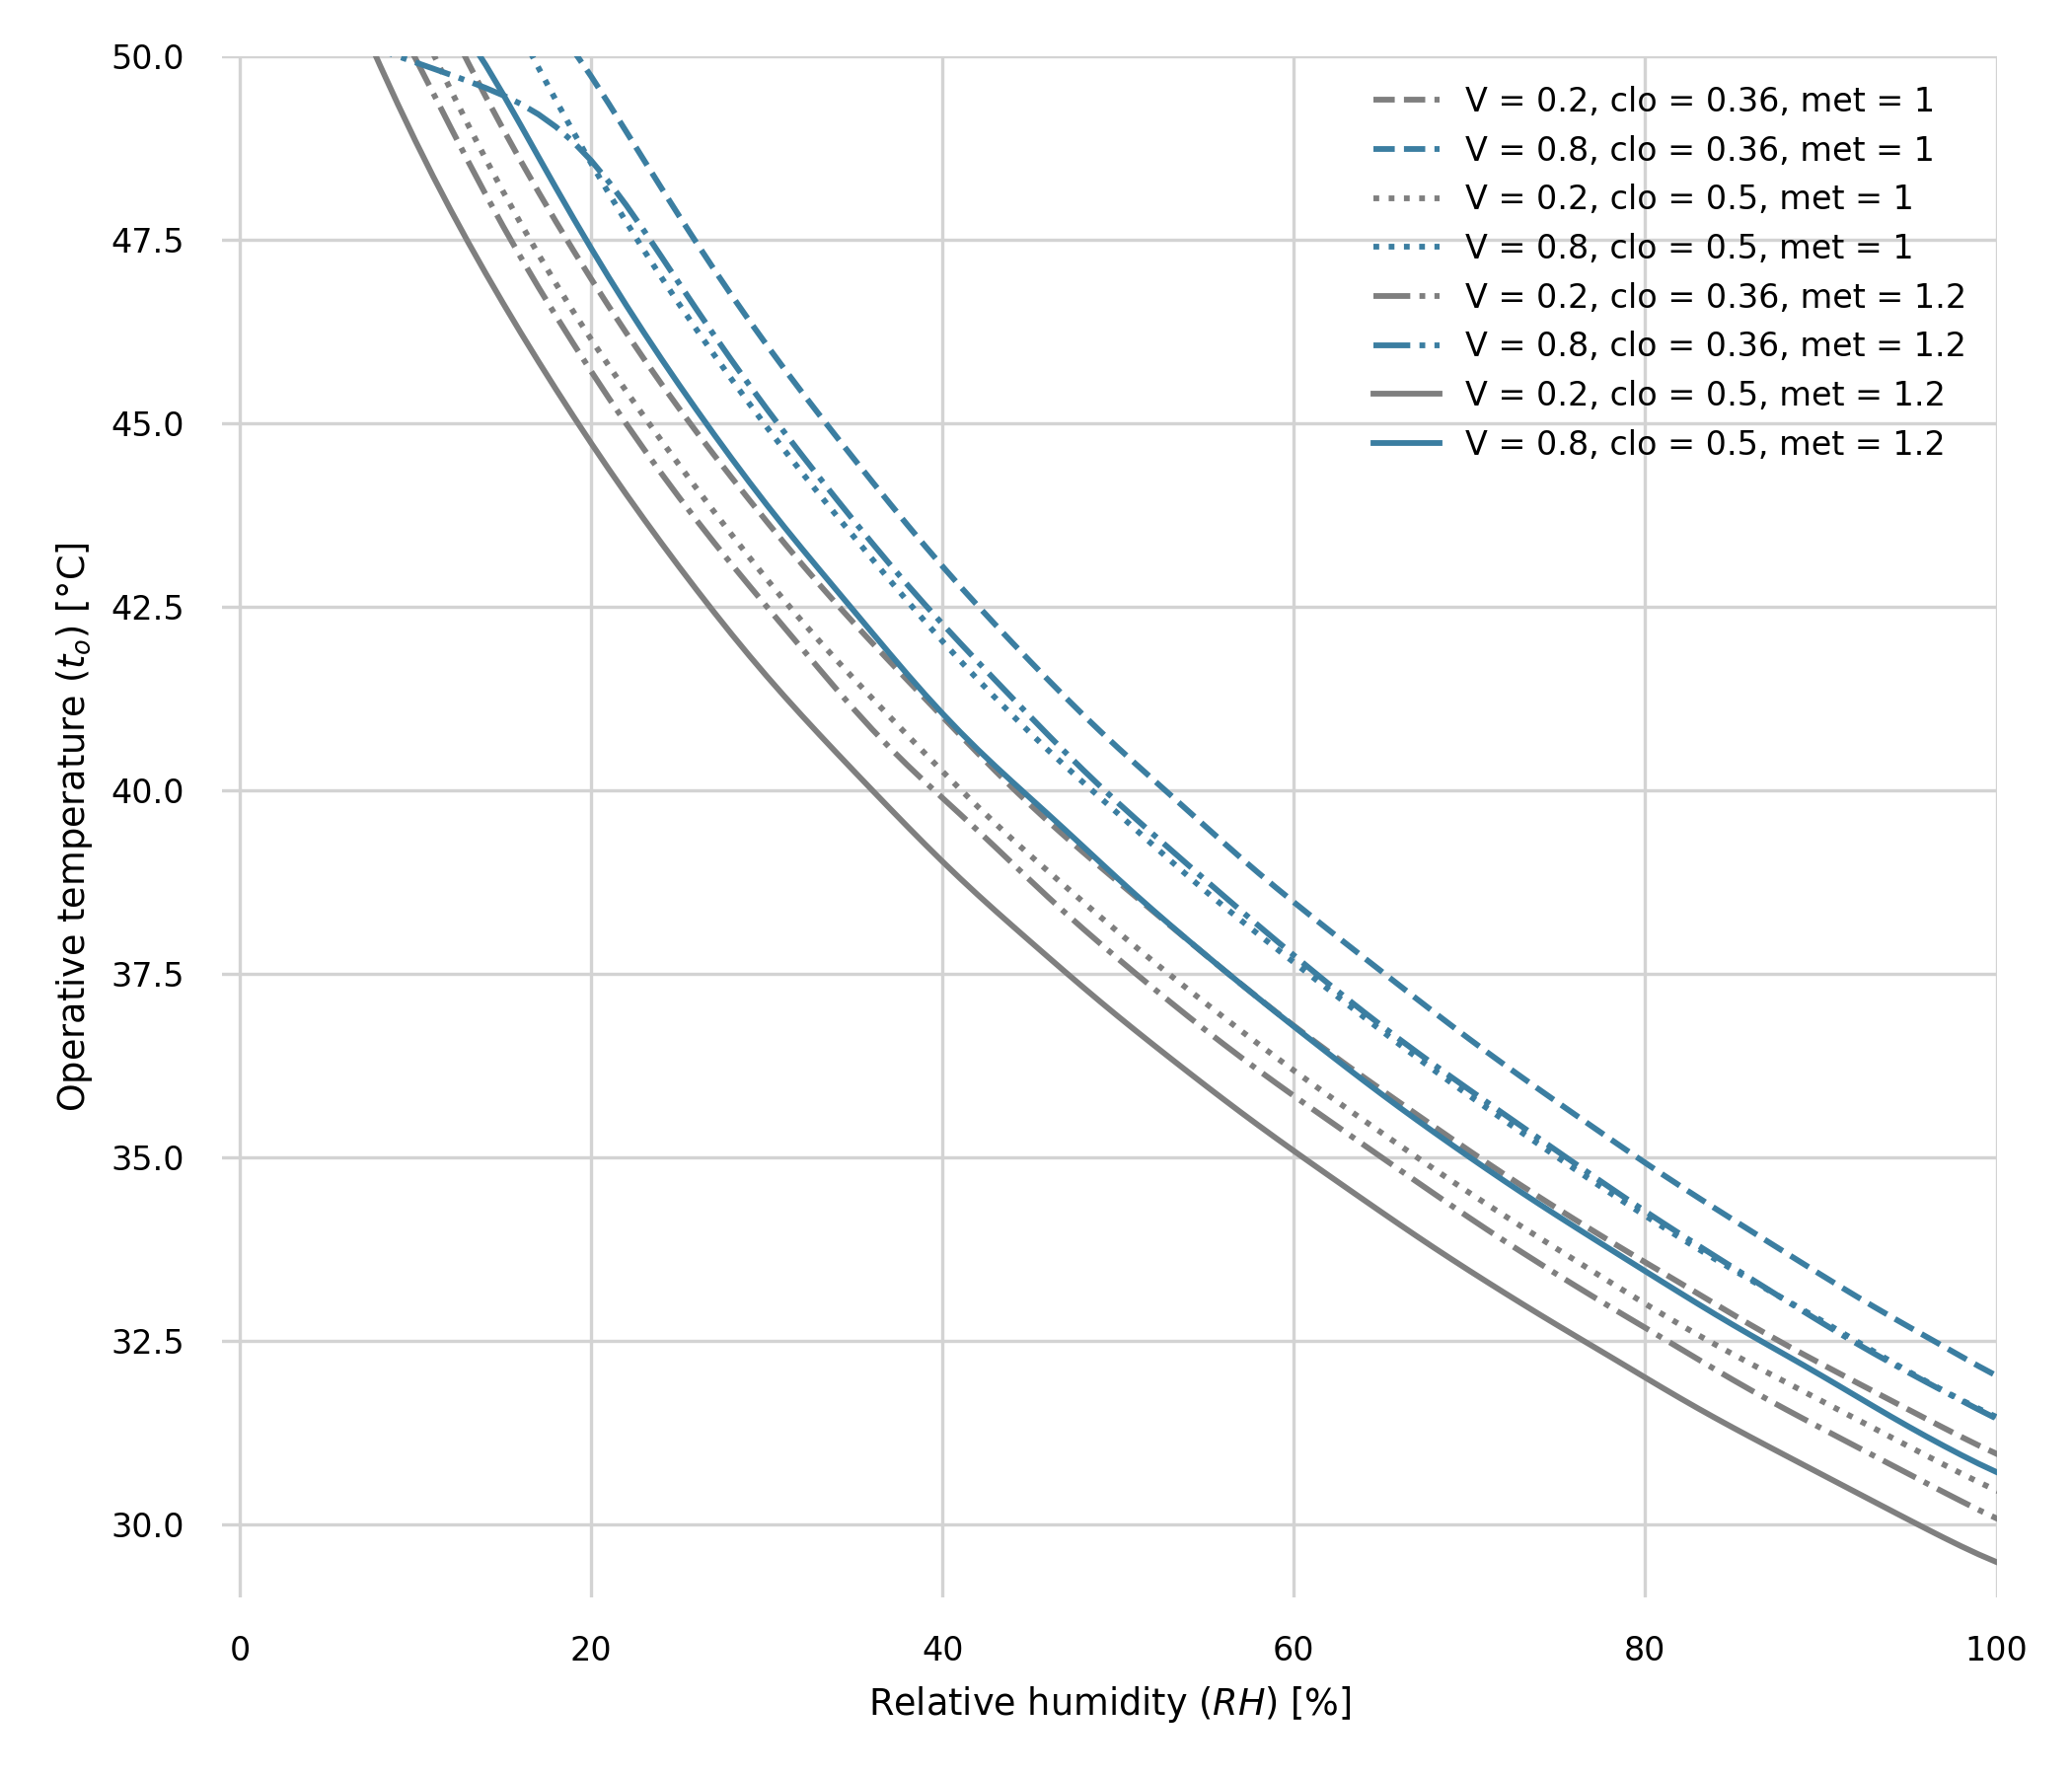
\includegraphics[width=\textwidth]{figures/met_clo}
    \caption{Each line demarcates how different combinations of personal factors (e.g., \ac{met}, \ac{clo}) and environmental factors affect the point above which the body cannot longer dissipate all the endogenous and exogenous heat gains}
    \label{fig:met_clo}
\end{figure}

The environmental conditions above which the use of elevated air speeds would be detrimental according to or model is shown in Figure~\ref{fig:energy_storage_delta}.
We used a red filling to highlight the region in which electrical fans should not be used, while we used a green background to depict when elevated air speed can safely be used to cool the human body.
We used a blue background to show the area in which fans are effective tool to prevent heat stress only if are used in combination with evaporative cooling technologies.
\todo{shall we remove this sentence?}
We also plotted the lines above which thermal stress is expected to occur (see Figure~\ref{fig:comparison_air_speed} for more details). 
For a specific value of \ac{rh}, as the value of \ac{v} increases the critical temperature at which thermal stress would occur also increases, however, at the same time the temperature above which fans should not be used also decreases by a greater amount.

We used a scatter plot to visualize the maximum extreme weather conditions recorded worldwide in more than 5000 stations.
Each dot represents the most extreme heat event recorded in each location.
Based on the climate data obtained from the 2017 ASHRAE Handbook--Fundamentals we determined that in approximately 73~\% of the locations thermal stress should not occur even without air movement, however, this number increases to 90~\% and 94~\% when \ac{v} is increased to 0.8~m/s and 4.5~m/s, respectively.
The use of fans during heatwaves would, therefore, be beneficial in the great majority of the locations worldwide.
With the exception of 29 locations where the use of \ac{v} higher than 0.8~m/s would be detrimental for the human body, and 7 locations where elevated air movement should not be used in any scenario.

% https://advances.sciencemag.org/content/6/19/eaaw1838

% todo report estimated sweat heat lossess too, either using a table or a heatmap

\begin{figure}[thb!]
    \centering
    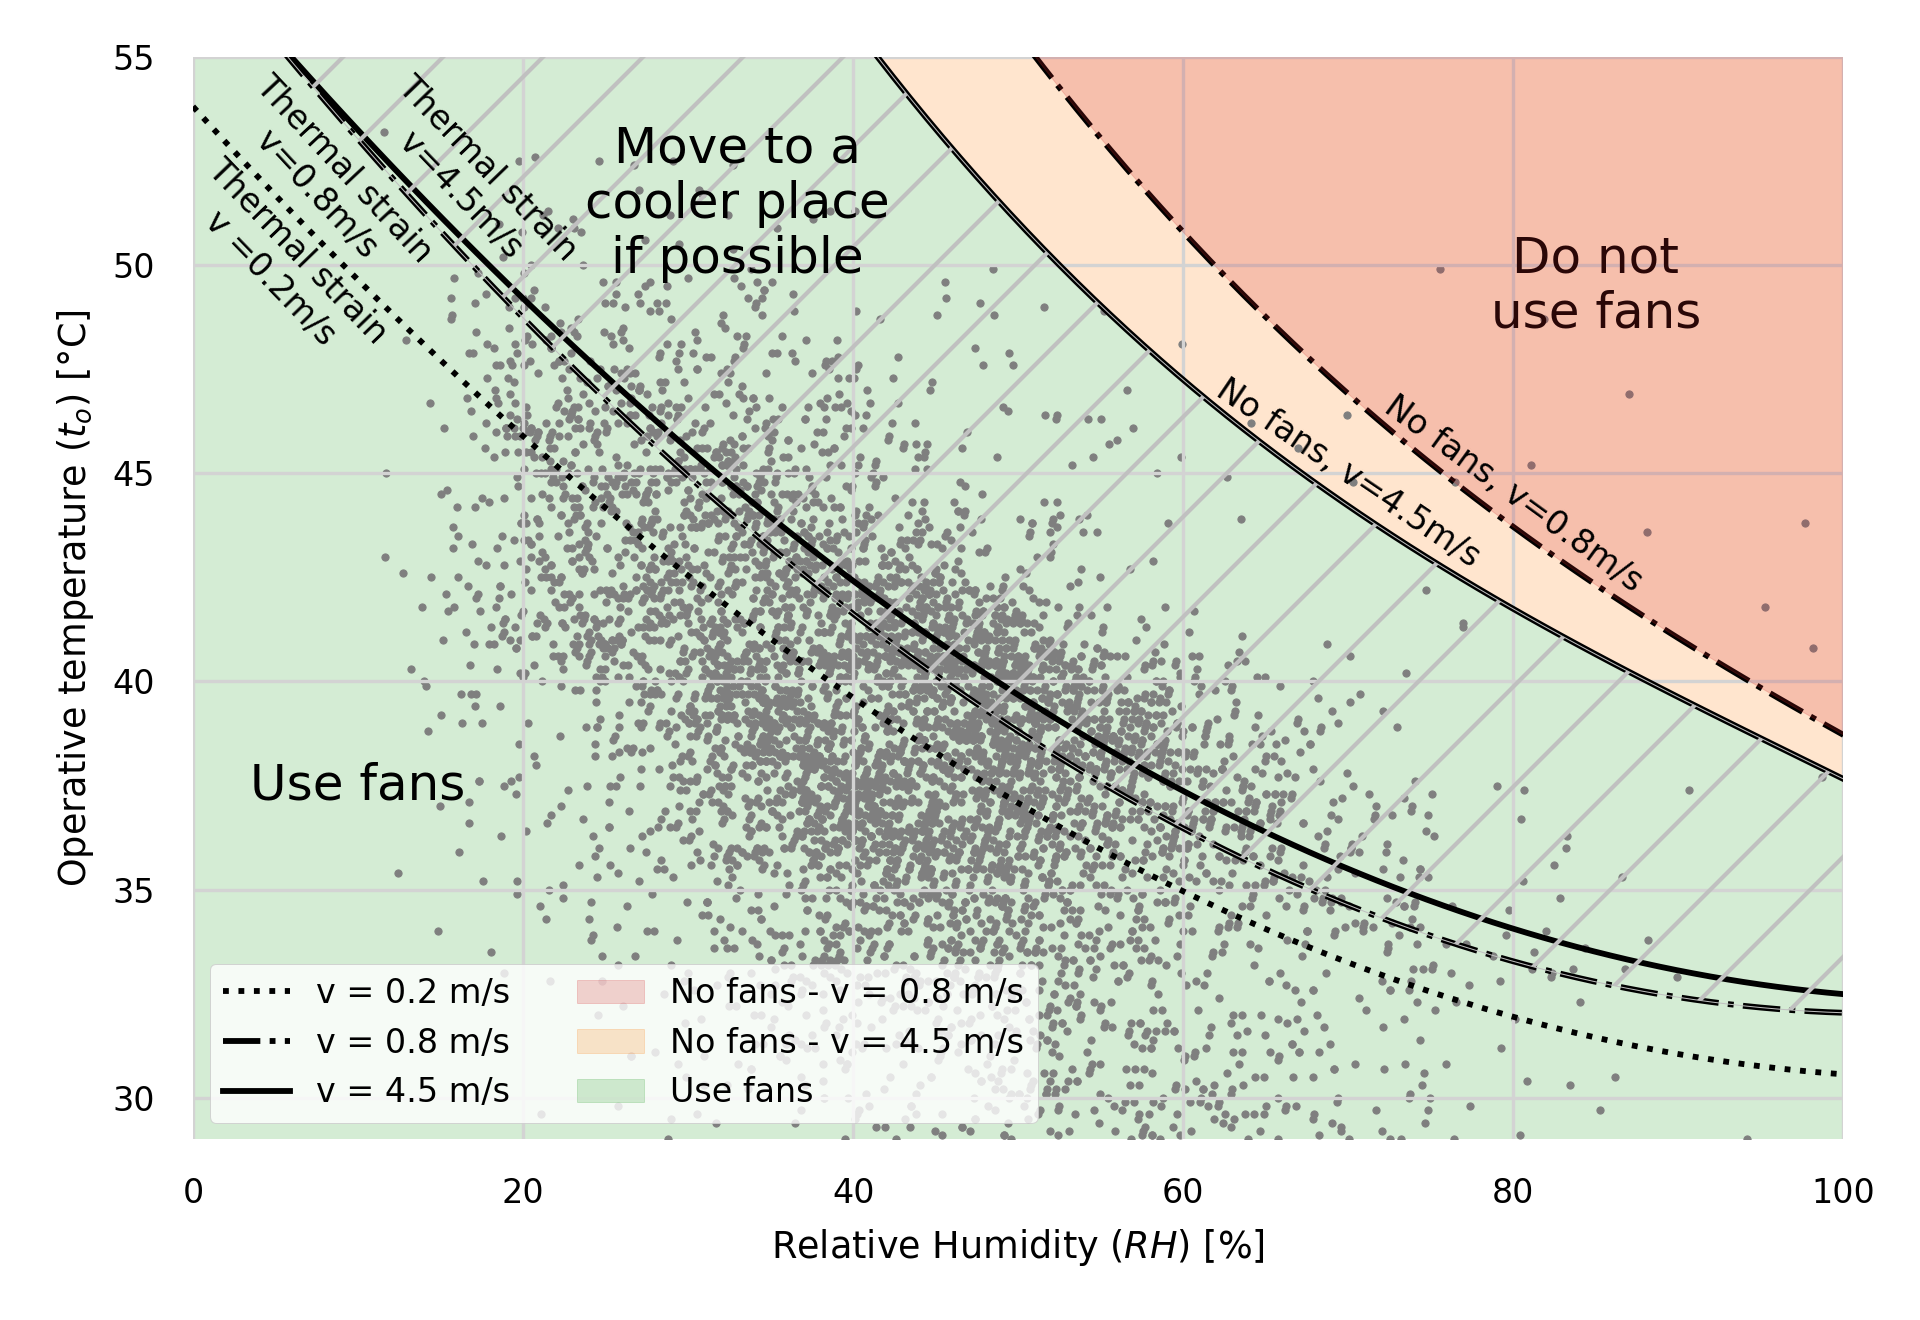
\includegraphics[width=\textwidth]{figures/use_fans}
    \caption{The green area shows the environmental conditions in which the use of fans is beneficial since they provide additional cooling to the human body.
    In the hatched area, while the use of fans it is still beneficial, people are most likely to suffer from heat strain.
    The red area demarcates the region in which electrical fans should not be used.
    The dots show the maximum extreme climate conditions recorded over the last 10 years in more than 5000 locations worldwide.
     These results were calculated assuming \ac{t-r} = \ac{t-db}, \ac{clo} = 0.5~clo, \ac{met} = 1.1~met.
    The red line depicts the current upper temperature limit above which many standards discourage people from using electrical fans.}
    \label{fig:energy_storage_delta}
\end{figure}

% todo compare results in the above figure with the results obtained by Gagnon

To better quantify how many people would benefit from the use of electrical fans we combined the city population with the weather data.
The former contained data from the 115 most populous cities worldwide.
We then plotted the data in Figure~\ref{fig:map-population-temperature}.
Each marker shows where the city is located, the dot size is proportional to the number of people living in that urban area, while the color shows the extreme \ac{t-db} recorded in that city.
In 2020, a total of approximately 650 million people (8~\% percent of global population) lived in the urban agglomerate of the 115 largest cities.
In 95 of them, \ac{t-db} higher than 35~$^{\circ}$C\@ were recorded and these cities had a total population of approximately 550 million people.

% todo make sure the area of the marker is proportial to the population and not its radius
\begin{figure}[thb!]
    \centering
    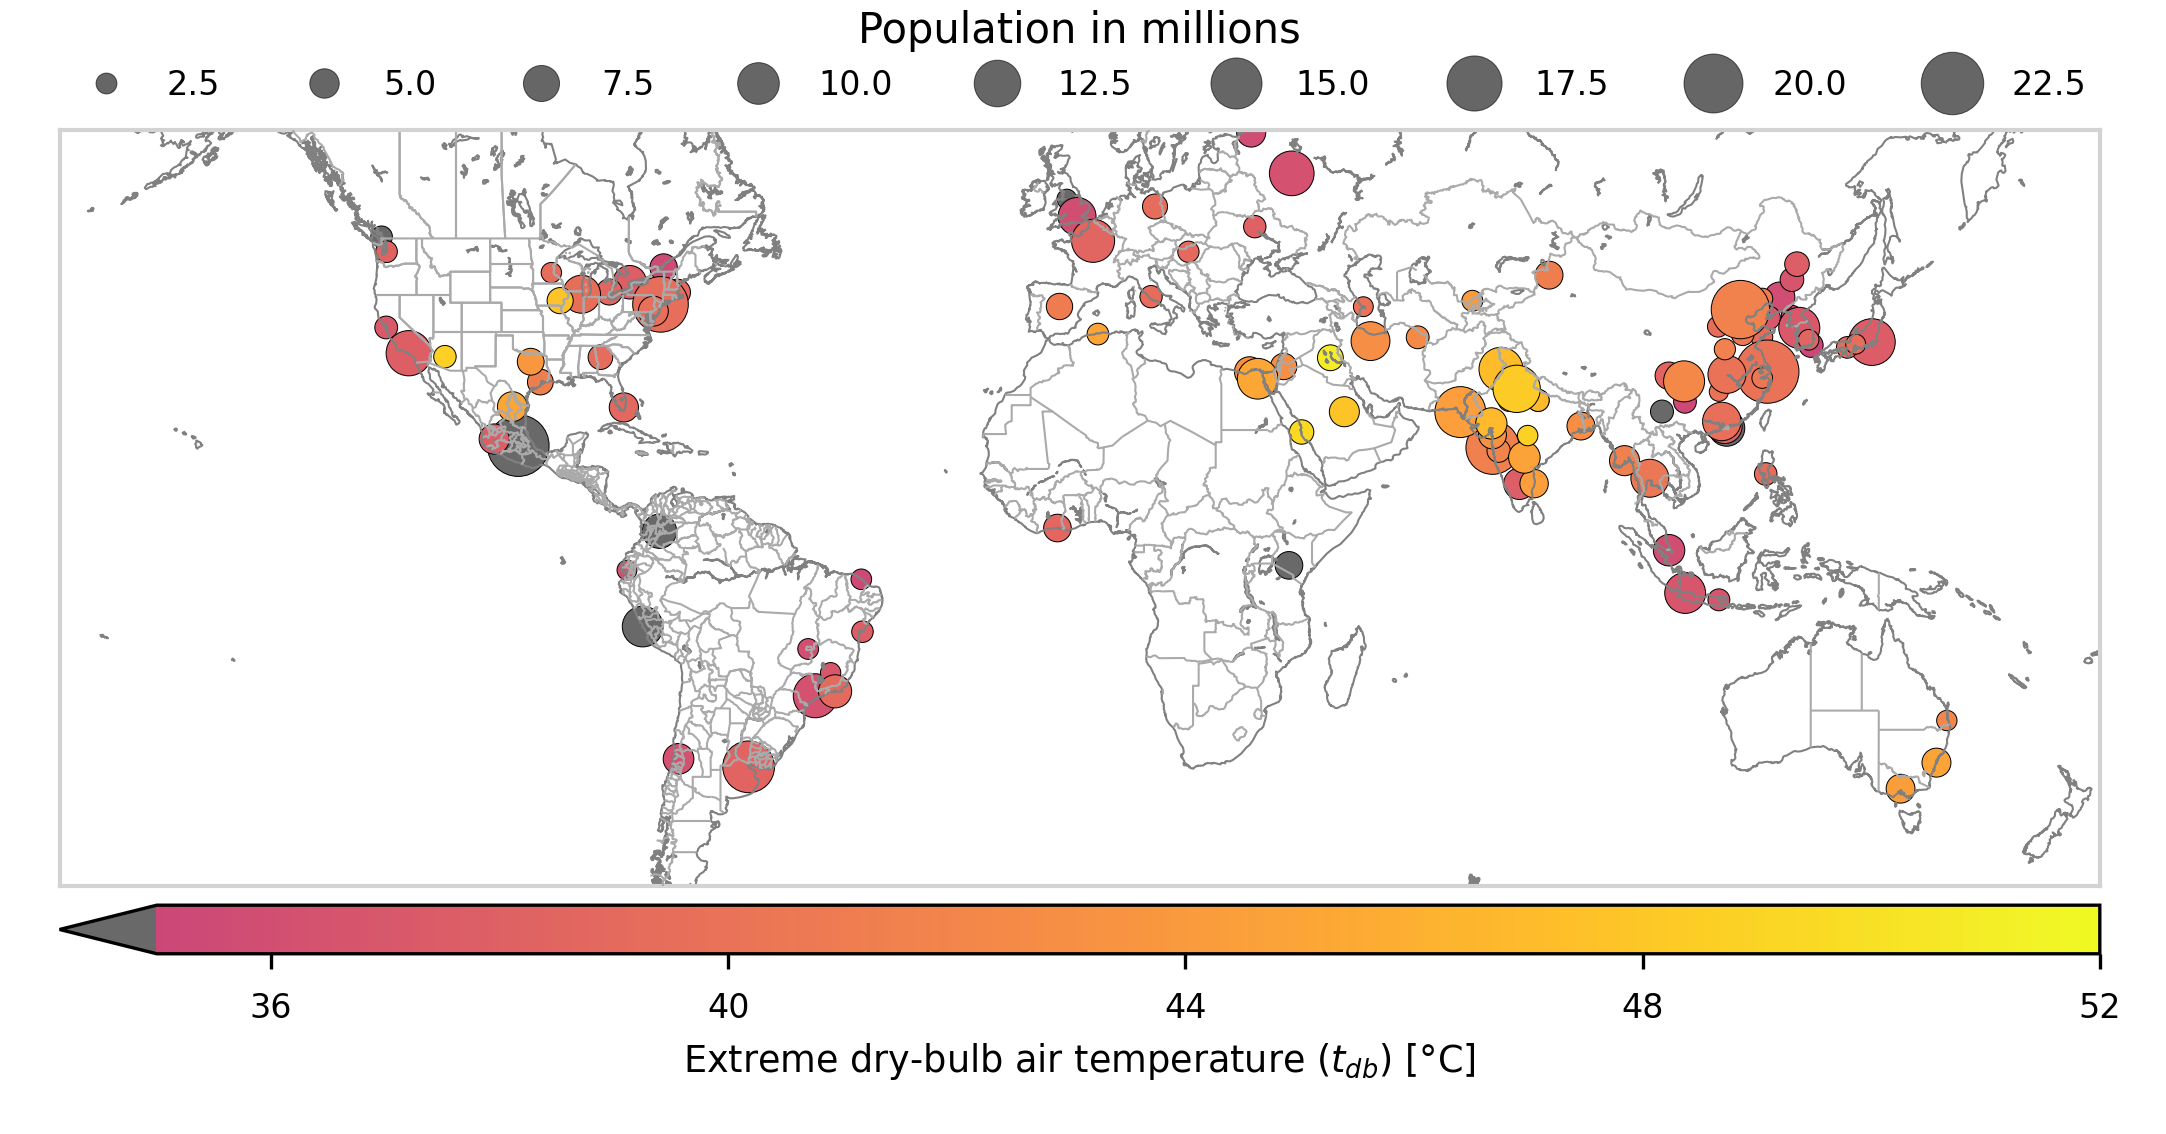
\includegraphics[width=\textwidth]{figures/map-population-temperature}
    \caption{Most populous 115 cities worldwide}
    \label{fig:map-population-temperature}
\end{figure}

We estimated that in all the 115 most populous cities the use of electrical fans would be beneficial for healthy adults seated quietly (\ac{met}~=~1.0~met) and wearing a value of \ac{clo} equal to 0.36~clo.
The \mycite{GaggeSET} model predicted that healthy adults living in 41 cities (approximately 230 million inhabitants) should not experience heat strain even without increasing air movement.
However, they should still be encouraged in using electrical fans to improve thermal comfort conditions in a energy efficient way.
An additional 167 million people would possibly avoid heat strain by simply elevating air speed up to 0.8~m/s.

\begin{figure}[thb!]
    \centering
    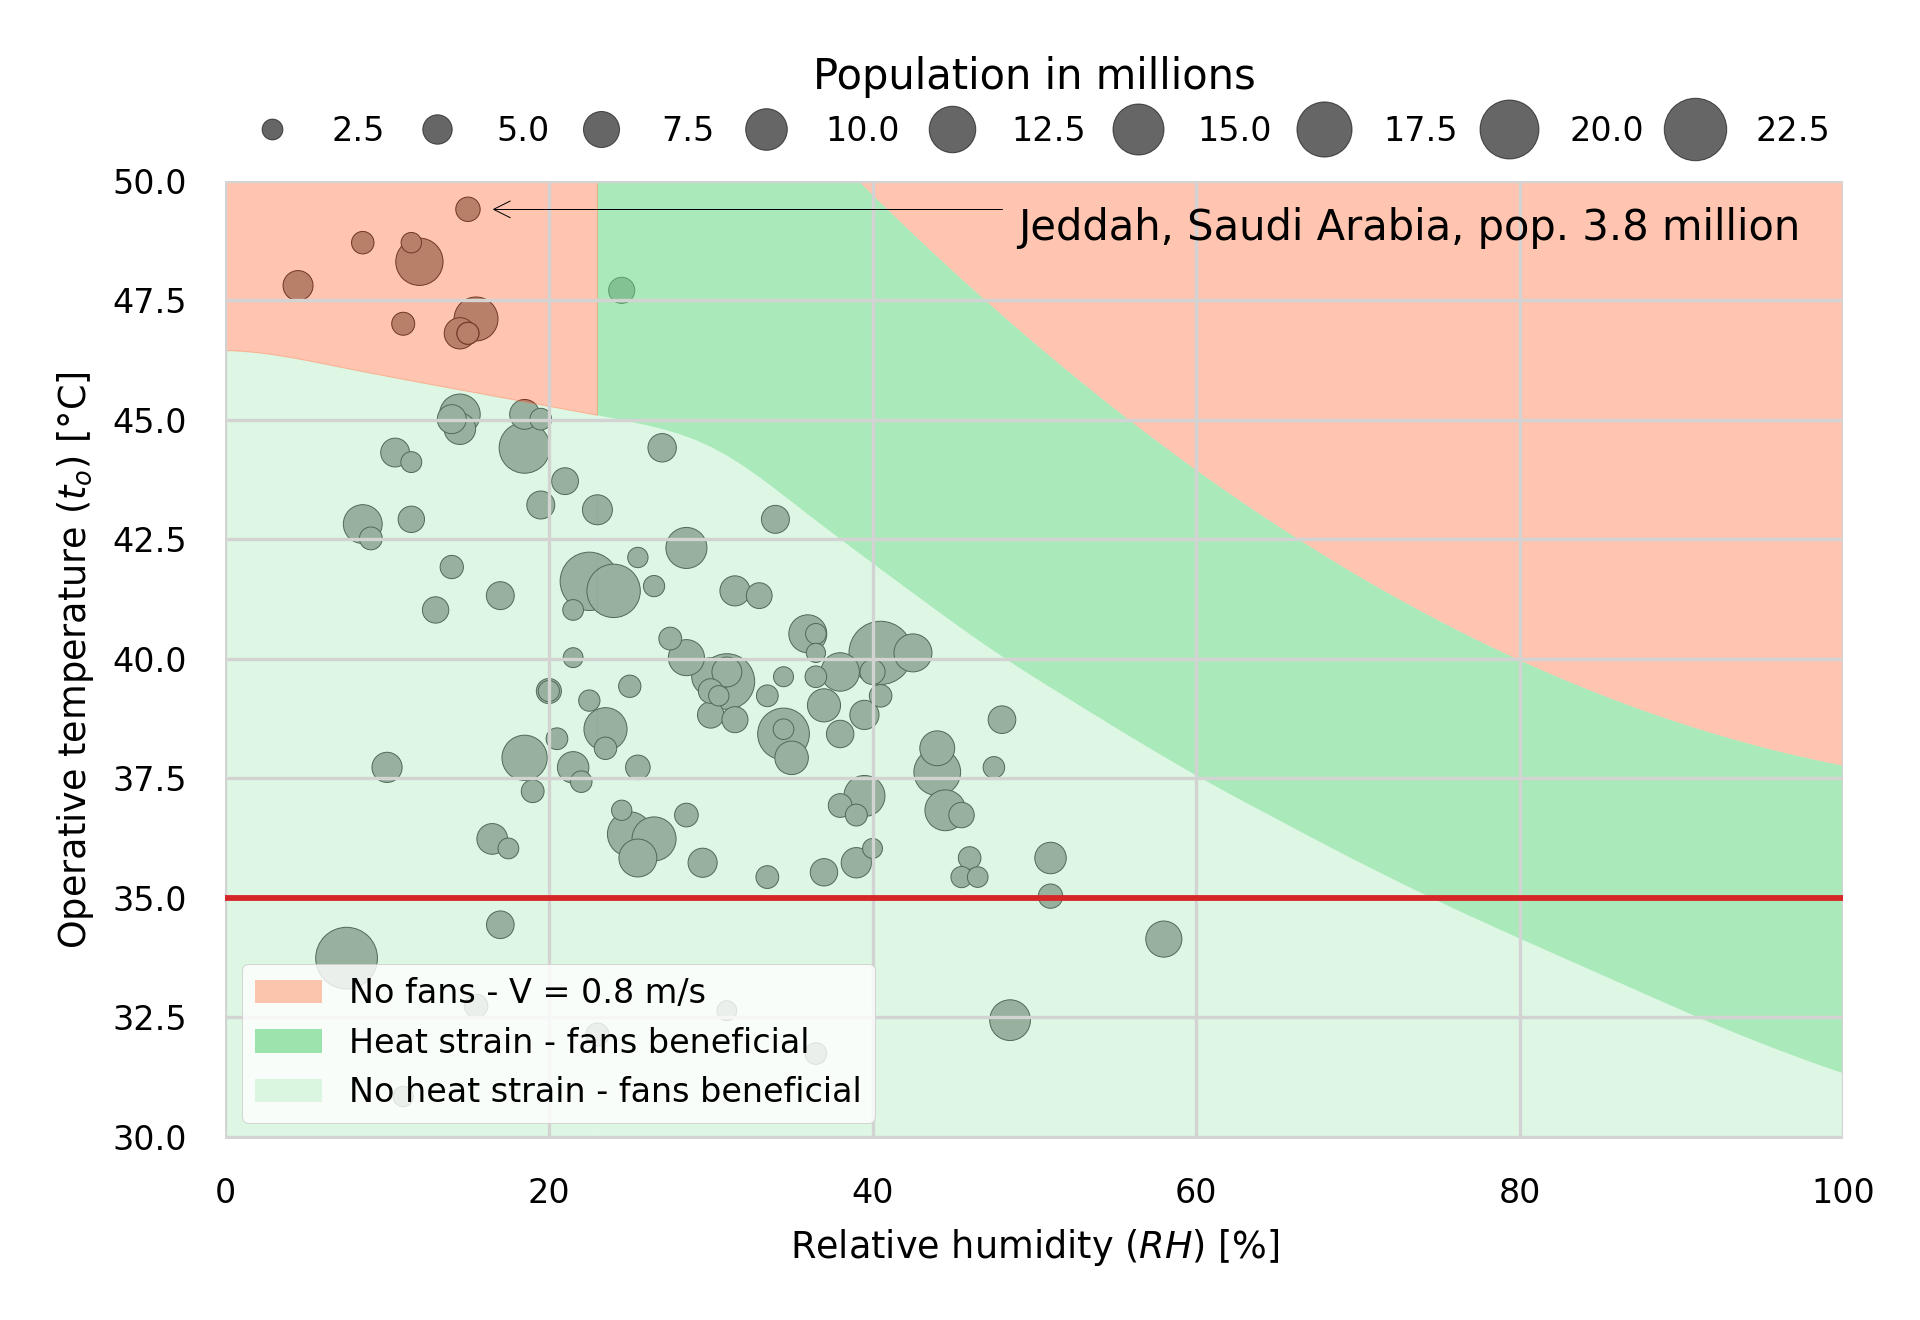
\includegraphics[width=\textwidth]{figures/use_fans_and_population}
    \caption{Environmental conditions under which the use of the electrical fans is beneficial, for more information on how to interpret the Figure please refer to the caption of Figure~\ref{fig:energy_storage_delta}.
    Each dot shows the maximum extreme climate conditions recorded over the last 10 years in each of the 115 most populous cities worldwide.
     These results were calculated assuming \ac{t-r}~=~\ac{t-db}, \ac{clo}~=~0.35~clo, \ac{met}~=~1.0~met.}
    \label{fig:use_fans_and_population}
\end{figure}